\begin{frame}{TODO}
    \begin{figure}[t]
        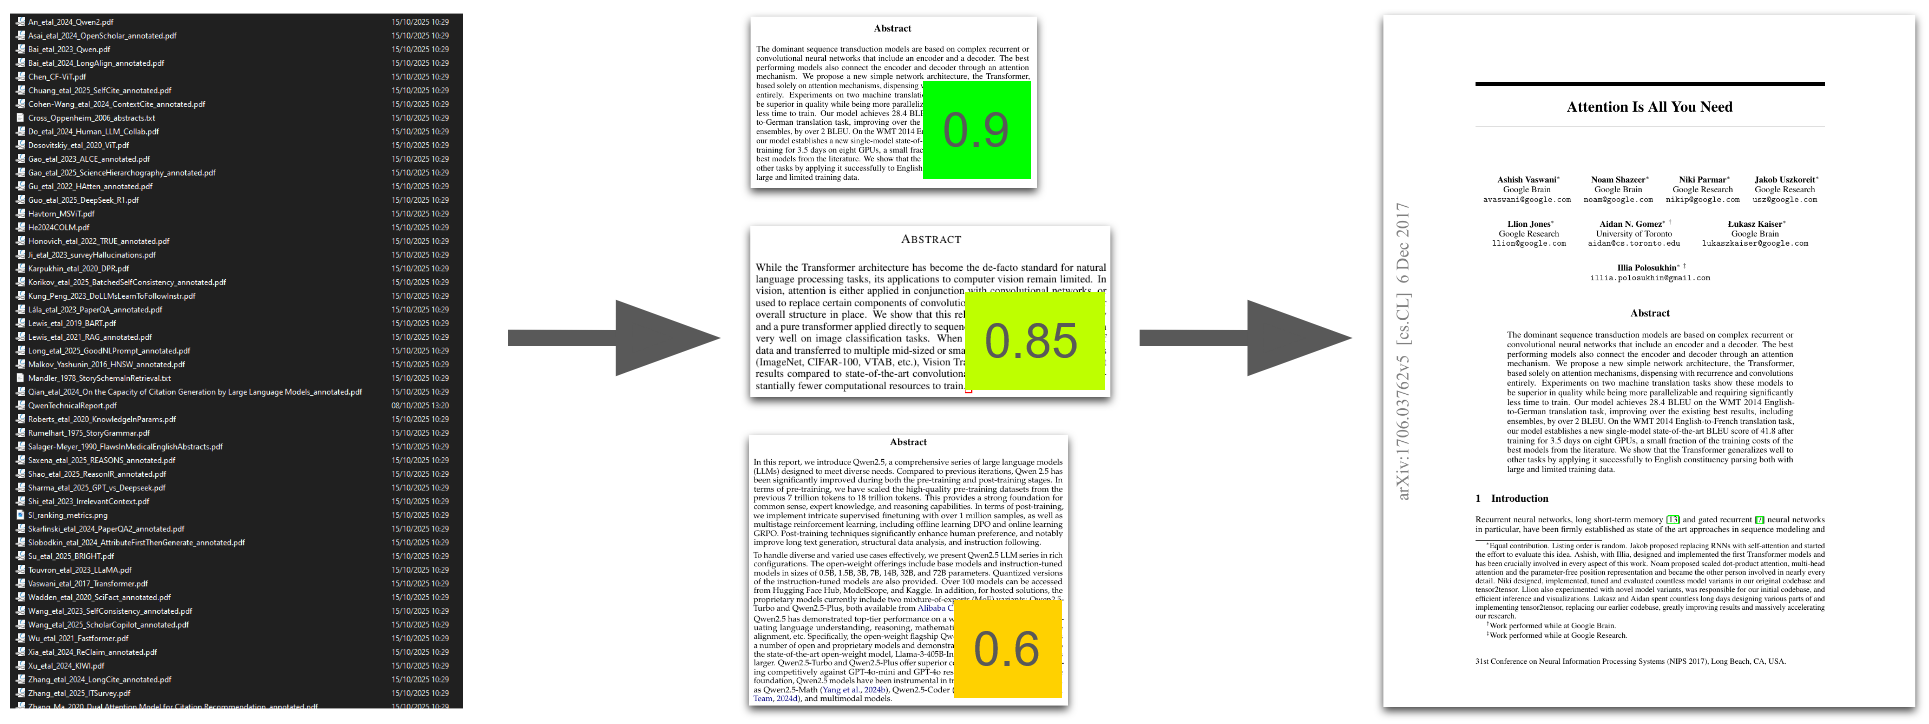
\includegraphics[width=\textwidth]{images/schematic_sc.png}
    \end{figure}
\end{frame}

\begin{frame}{TODO}
    \begin{figure}[t]
        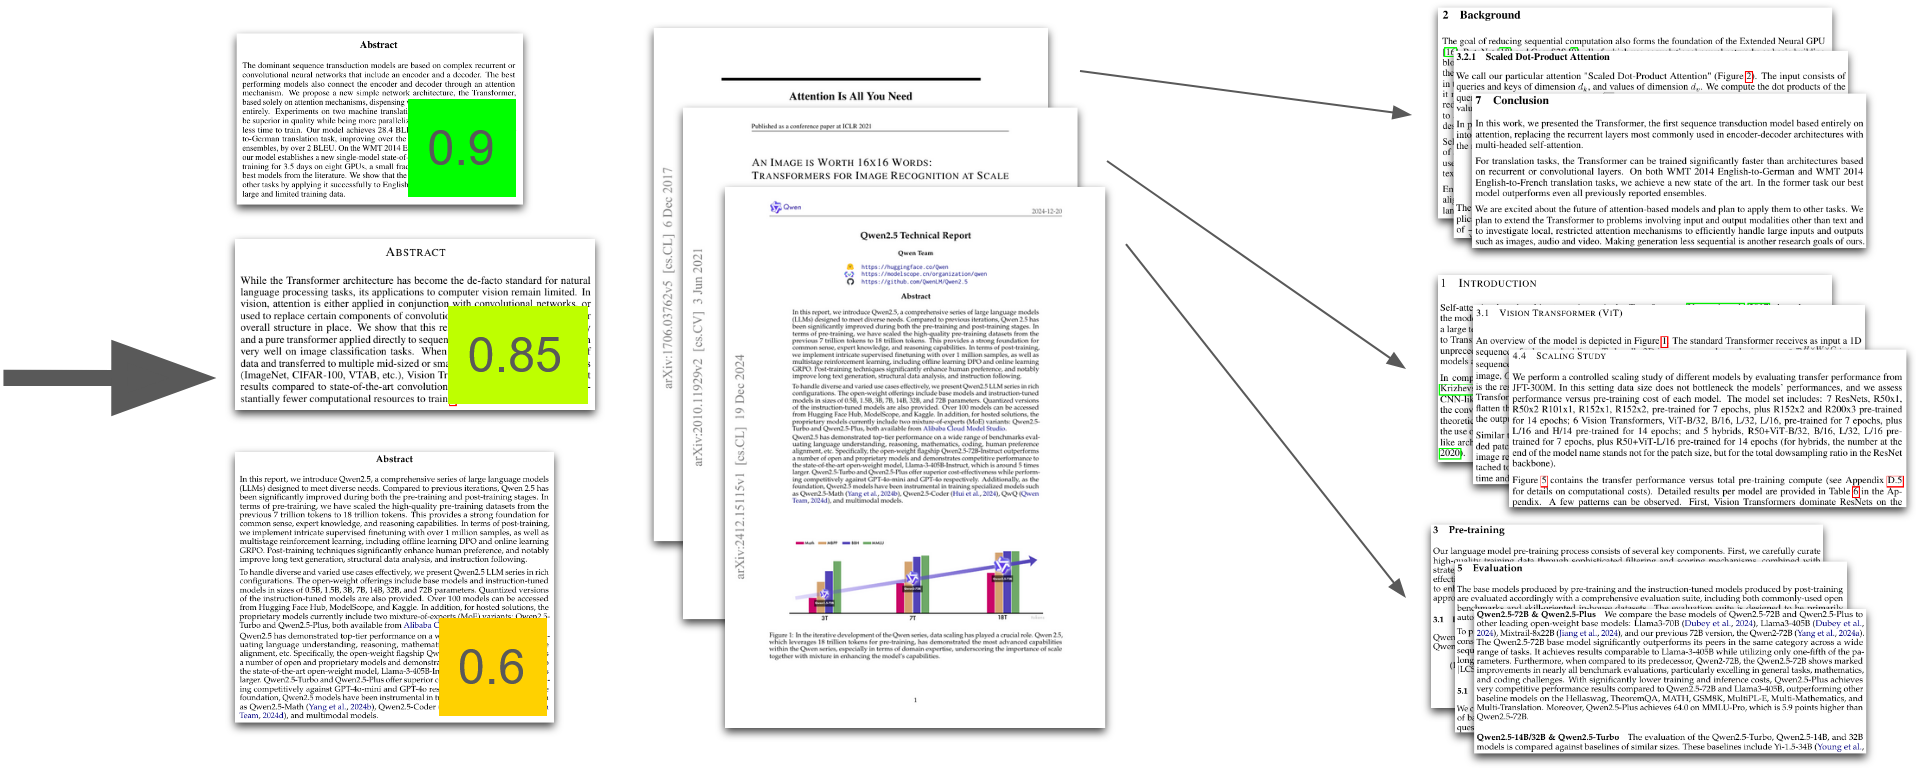
\includegraphics[width=\textwidth]{images/schematic_pr1.png}
    \end{figure}
\end{frame}

\begin{frame}{TODO}
    \begin{figure}[t]
        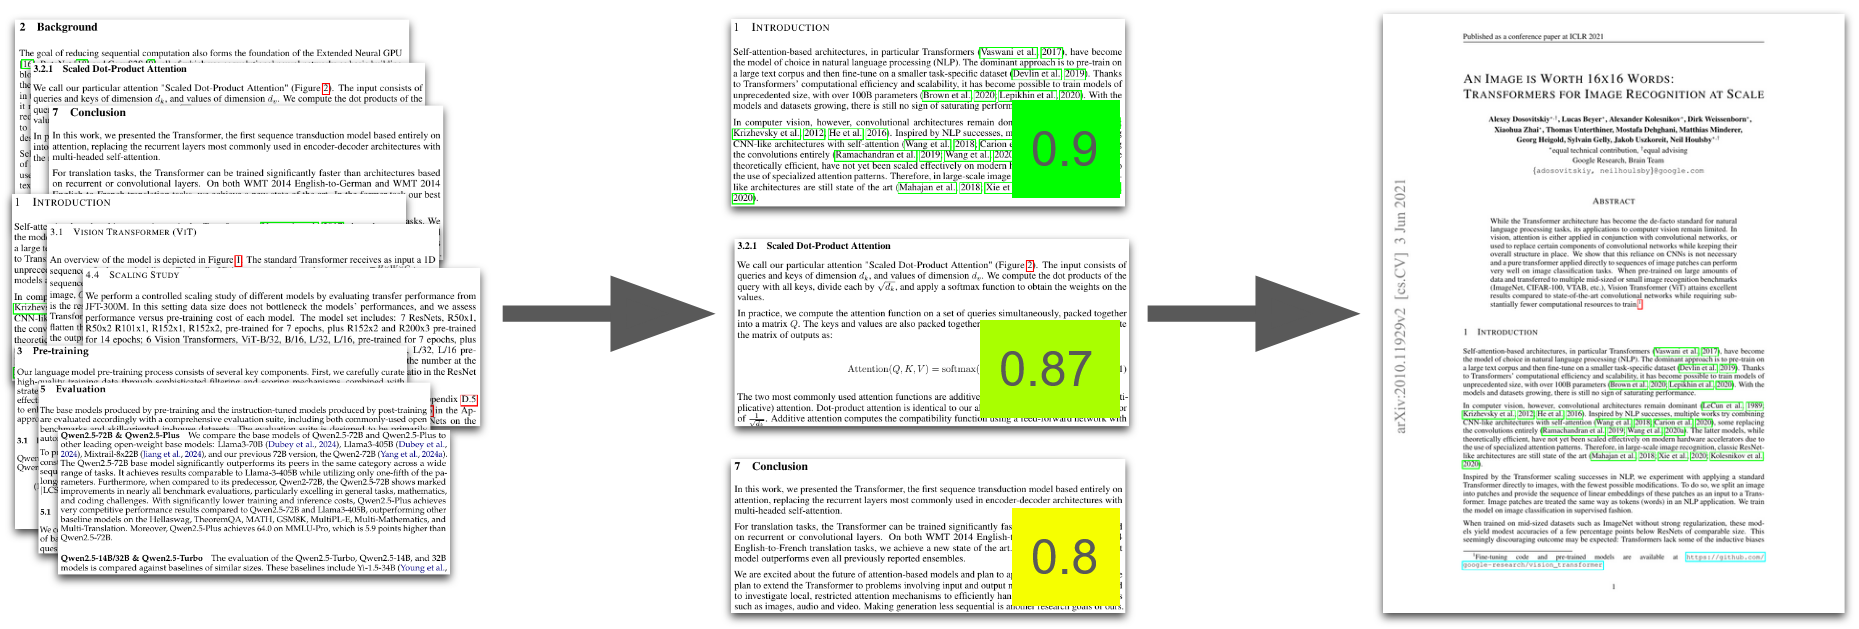
\includegraphics[width=\textwidth]{images/schematic_pr2.png}
    \end{figure}
\end{frame}

\begin{frame}{Citation Recall Performance}
    \begin{columns}
        \begin{column}{0.5\textwidth}
            \begin{figure}[t]
                
\includegraphics[width=1.001\textwidth, trim={2.6cm 0 0 0.35cm}, clip]{images/plot_retrieval_masked.pdf}
            \end{figure}
        \end{column}
        \begin{column}{0.5\textwidth}
            \begin{figure}[t]
                
\includegraphics[width=1.001\textwidth, trim={2.6cm 0 0 0.35cm}, clip]{images/plot_retrieval_with_abstracts.pdf}
            \end{figure}
        \end{column}
    \end{columns}
\end{frame}

\begin{frame}{Recall@$k$ decline towards small $k$}
    \begin{table}[t]
        \begin{center}
            \resizebox{\textwidth}{!}{\begin{tabular}{llccccc}
                \textbf{Model} & \textbf{Dataset} & \mono{intro+relwork} & \mono{methods} & \mono{experiments} & \mono{conclusion} & $\Sigma$ \\
                \hline
                \hline
                SC & \mono{masked} & $-0.06$ & $-0.04$ & $-0.09$ & $-0.07$ & $-0.26$\\
                \hline
                SC & \mono{with-abstracts} & $-0.05$ & $-0.06$ & $-0.07$ & $-0.06$ & $-0.24$\\
                \hline
                SC+PR & \mono{masked} & $-0.03$ & $-0.03$ & $-0.05$ & $-0.05$ & \textbf{-0.16}\\
                \hline
                SC+PR & \mono{with-abstracts} & $-0.04$ & $-0.04$ & $-0.03$ & $-0.04$ & \textbf{-0.15}\\
                \hline
            \end{tabular}}
        \end{center}
        \caption{Cumulative Recall@$k$ difference from $k=10$ over $k=5$ to $k=1$.}
        \label{tab:cumulative_recall_loss}
    \end{table}
\end{frame}

\begin{frame}{Why is the recall for \mono{experiments} so much higher?}
    \begin{table}[t]
    \begin{center}
        \resizebox{\textwidth}{!}{\begin{tabular}{lcccc}
             & \mono{intro+relwork} & \mono{methods} & \mono{experiments} & \mono{conclusion} \\
            \hline
            \hline
            last token in abstract & $0.08$ & $0.12$ & \textbf{0.22} & $0.11$ \\
            \hline
        \end{tabular}}
    \end{center}
    \caption{Fraction of cases where the last token before the citation appears in the abstract of the cited document.}
    \label{tab:last_token}
\end{table}
\end{frame}

\begin{frame}{Correct Retrieval Overlap}
    \begin{table}[t]
        \resizebox{\textwidth}{!}{\begin{tabular}{llccccc}
            \textbf{Dataset} & \textbf{Metric} & \mono{intro+relwork} & \mono{methods} & \mono{experiments} & \mono{conclusion} & $\mu$ \\
            \hline
            \hline
            \mono{masked} & Recall@$10$ & $0.91$ & $0.97$ & $0.98$ & $0.91$ & $0.943$\\
            \hline
            \mono{masked} & Recall@$5$ & $0.94$ & $0.94$ & $0.96$ & $0.94$ & $0.945$\\
            \hline
            \mono{masked} & Recall@$1$ & \textbf{0.79} & 0.89 & \textbf{0.88} & $0.88$ & \textbf{0.86}\\
            \hline
            \mono{with-abstracts} & Recall@$10$ & $0.9$ & $0.93$ & $0.96$ & $0.95$ & $0.935$\\
            \hline
            \mono{with-abstracts} & Recall@$5$ & $0.86$ & $0.97$ & $0.95$ & $0.89$ & $0.918$\\
            \hline
            \mono{with-abstracts} & Recall@$1$ & $0.87$ & \textbf{0.87} & $0.93$ & \textbf{0.84} & $0.878$\\
            \hline
        \end{tabular}}
        \caption{Fraction of correct retrievals by ScholarCopilot given correct retrieval by the PR module.}
        \label{tab:successful_retrieval_overlap}
    \end{table}
\end{frame}

\begin{frame}{TODO}
    TODO
\end{frame}

\begin{frame}{TODO}
    TODO
\end{frame}

\begin{frame}{TODO}
    TODO
\end{frame}

\begin{frame}{TODO}
    TODO
\end{frame}

\begin{frame}{TODO}
    TODO
\end{frame}

\begin{frame}{TODO}
    TODO
\end{frame}

\begin{frame}{TODO}
    TODO
\end{frame}

\begin{frame}{TODO}
    TODO
\end{frame}

\begin{frame}{TODO}
    TODO
\end{frame}

\begin{frame}{TODO}
    TODO
\end{frame}